\documentclass[british,titlepage,twoside]{ntnuthesis}

\title{Paving the Way for Enhanced Situational Awareness in the Maritime Domain: 
Designing and Ensembling a Sensor Rig for Multi-Sensor Data Set Acquisition}
\shorttitle{Sensor Rig for Multi-Sensor Data Set Acquisition}
\author{Emil Martens}
\shortauthor{Emil Martens}
\date{Spring 2023}
\addbibresource{thesis.bib}


% --------------------
% ----- Commands -----
% --------------------
\newcommand{\code}[1]{\hspace{-.3em}\mintinline{text}{#1}\hspace{-.3em}\xspace}
\newcommand{\todo}{\textcolor{red}{Todo}\xspace}
\newcommand{\review}{}
% \newcommand{\review}{\textcolor{green}{Draft Complete}\\}
\newcommand{\done}{}
% \newcommand{\done}{\textcolor{olive}{Done}\\}
% \makeglossaries

\setabbreviationstyle[acronym]{long-postshort-user}
\glssetcategoryattribute{acronym}{nohyperfirst}{true}
\setabbreviationstyle{short-nolong}
\makeglossaries

% --------------------
% ---- Glossaries ----
% --------------------
\newglossaryentry{asyncio}{name=Asyncio, description={A Python library for asynchronous code.}}
\newglossaryentry{stim}{name=STIM300, description={A MEMS-based \gls{imu}}}
\newglossaryentry{f9p}{name=F9P, description={A Global Navigation Satellite System (GNSS) receiver manufactured by u-blox.}}

% --------------------
% ----- Acronyms -----
% --------------------
\newacronym{asv}{ASV}{Autonomous Surface Vehicle}
\newacronym{dolp}{DoLP}{Degree of Linear Polarization}
\newacronym{aolp}{AoLP}{Angle of Linear Polarization}
\newacronym{sitaw}{SITAW}{Situational Awareness}
\newacronym{poe}{PoE}{Power over Ethernet}
\newacronym{pps}{PPS}{Pulse Per Second}
\newacronym{cpfa}{CPFA}{Color-Polarization Filter Array}
\newacronym{utc}{UTC}{Coordinated Universal Time}
\newacronym{imu}{IMU}{Inertial Measurement Unit}
\newacronym{tov}{TOV}{Time of Validity}
\newacronym{tm2}{TM2}{Time mark data}
\newacronym{gnss}{GNSS}{Global Navigation Satellite System}
\newacronym{ptp}{PTP}{Precision Time Protocol}

% \glsaddall
% \makenoidxglossaries

% \glsunset{cpu}
\glsunset{gnss}
\glsunset{imu}
\glsunset{tm2}
\glsunset{utc}

% --------------------
% ----- Shortcuts ----
% --------------------

 
% \oneside
% 
\emergencystretch=1em
% \includeonly{chapters/10_intro/__include__}
% \includeonly{chapters/30_debayer_in_cuda/__include__}

\begin{document}

\includepdf{chapters/10_intro/frontpage.pdf}
\tableofcontents
% \listoffigures
% \listoftables
% \lstlistoflistings 
\pagebreak

\chapter{Polarization Cameras}
\label{chap:cameras}
This chapter presents the special type of polarization cameras used, explains how they work, and why they are particularly well suited for detection in marine environments.
Furthermore, it covers how to interact with the \cams through their \gls{api} and how the network adapters have been configured to achieve reliable $2Gb/s$ throughput from the \cams.





\section{Polarization of Light}
This section is based on Section 1.7 of University Physics Volume 3 \cite[30-33]{lingUniversityPhysicsVolume2016}.
Light is an electromagnetic (EM) wave with oscillating electric and magnetic fields perpendicular to its direction of propagation.
The specific orientation of these oscillations is referred to as polarization.
Natural light sources, such as the Sun, emit unpolarized light in which the electric fields have random orientations, encompassing various polarization directions.

Polarizing filters can transmit light waves with polarization aligned with the filter's orientation while blocking waves that are not aligned.
This behavior follows Malus's law, which describes the relationship between the intensity of polarized light transmitted through a polarizer and the angle between the polarization direction of the incident light and the orientation of the polarizer:
\begin{equation}
    I = I_0 cos^2 \theta
\end{equation}

\subsection{Polarization Properties of Reflected Light}
Unpolarized light becomes partially polarized when reflected off a surface \cite[34]{lingUniversityPhysicsVolume2016}.
This is the reason why sunglasses are commonly polarized, as they are designed to block reflected light from surfaces such as roads or water.
Figure \ref{fig:polarized_reflection} illustrates this phenomenon where the light gets partially polarized parallel to the surface (perpendicular to the plane of incidence).
At one particular angle of incidence, the reflected light is completely polarized parallel to the surface.
This angle is called the Brewster angle and is given by \cite{BrewsterAngle2023}:

\begin{equation}
    \theta_B = \arctan{\frac{n_2}{n_1}}
\end{equation}

\begin{figure}[H]
    \centering
    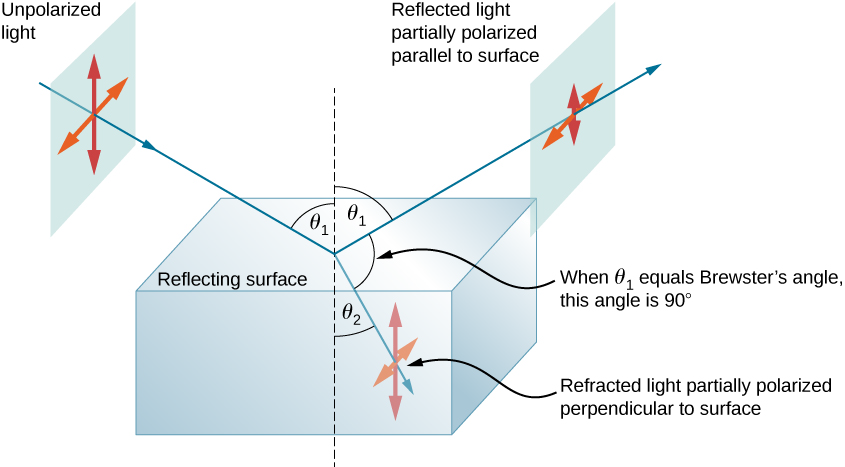
\includegraphics[width=\textwidth]{figures/polarization/reflaction.png}
    \caption{Polarization by reflection. \cite[Figure 1.38]{lingUniversityPhysicsVolume2016}}
    \label{fig:polarized_reflection}
\end{figure}


Any polarization state can be resolved as a sum of two orthogonal linear polarizations where one is perpendicular to the plane of incidence $R_\perp$ and the other is parallel to the plane of incidence $R_\parallel$ \cite{FresnelEquations2023}.
These two components are referred to as s-polarized and p-polarized light, respectively and their reflection coefficients are given by the Fresnel equations \cite{FresnelEquations2023}:

\begin{align}
    \centering
    R_\perp =         & \left|{\frac {n_{1}\cos \theta _1-n_{2}\cos \theta _2}{n_{1}\cos \theta _1+n_{2}\cos \theta _2}}\right|^{2} \\
    \\
    R_\parallel     = & \left|{\frac {n_{1}\cos \theta _2-n_{2}\cos \theta _1}{n_{1}\cos \theta _2+n_{2}\cos \theta _1}}\right|^{2}
\end{align}

Where  $\eta_1$ and $\eta_2$ are the refractive indices of the two media,
$\theta_i$ is the angle of incidence and $\theta_r$ is the angle of refraction.

Using the trigonometric identity $ \cos^2{\left(\theta_2 \right)} = 1- \sin^2{\left(\theta_2 \right)}$ and Snell's law $\eta_1 \sin{\left(\theta_1 \right)} = \eta_2 \sin{\left(\theta_2 \right)}$ the angle of refraction, $\theta_2$ can be removed, and the equations can be written as:

\begin{align}
    R_\perp =         & \left|{\frac {n_{1}\cos \theta _1-n_{2}{\sqrt {1-\left({\frac {n_{1}}{n_{2}}}\sin \theta _1\right)^{2}}}}{n_{1}\cos \theta _1+n_{2}{\sqrt {1-\left({\frac {n_{1}}{n_{2}}}\sin \theta _1\right)^{2}}}}}\right|^{2} \\
    \\
    R_\parallel     = & \left|{\frac {n_{1}{\sqrt {1-\left({\frac {n_{1}}{n_{2}}}\sin \theta _1\right)^{2}}}-n_{2}\cos \theta _1}{n_{1}{\sqrt {1-\left({\frac {n_{1}}{n_{2}}}\sin \theta _1\right)^{2}}}+n_{2}\cos \theta _1}}\right|^{2}
\end{align}


Inserting the refractive index of air, $n_1 = 1$, and the refractive index of water, $n_2 = 1.33$, the reflectance can be calculated and plotted as a function of the angle of incidence, $\theta_1$, alone as shown in Figure \ref{fig:brewster0}.


\begin{figure}[H]
    \centering
    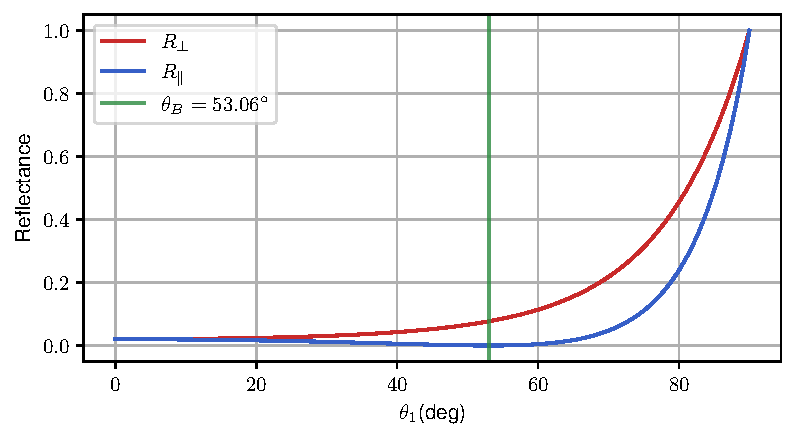
\includegraphics[width=\textwidth]{figures/pol_plots/brewster0.pdf}
    \caption{Reflectance of S and P polarized light of water as a function of the angle of incidence.}
    \label{fig:brewster0}
\end{figure}

The \gls{dolp} is the degree to which light is polarized and can be defined as the ratio between the difference and the sum of the two components:

\begin{align}
    DoLP= & \frac{\left | R_\perp - R_\parallel \right |}{R_\perp + R_\parallel}
\end{align}
\begin{figure}[H]
    \centering
    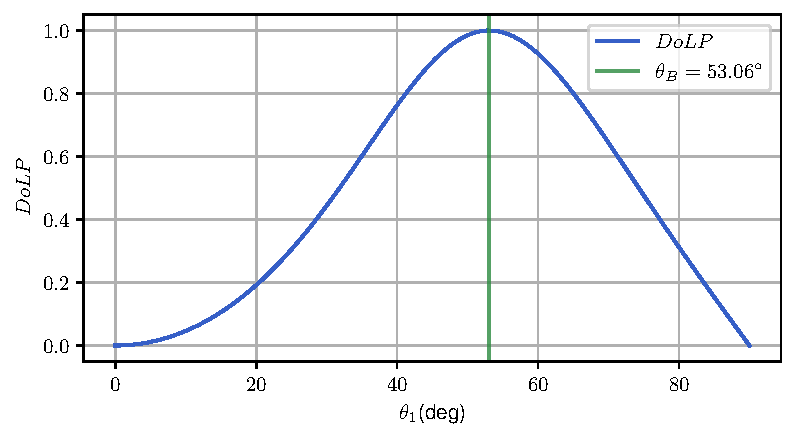
\includegraphics[width=\textwidth]{figures/pol_plots/brewster1.pdf}
    \caption{\gls{dolp} of light reflected off water as a function of the angle of incidence.}
    \label{fig:brewster1}
\end{figure}


\section{Color Polarization Filter Array Sensors}
In recent years, the development of microscopic polarization filters has enabled the production of camera sensors where each pixel has its own polarization filter, as illustrated in Figure \ref{fig:camera_crosstalk} \cite{lucidvisionlabsLUCIDGoingPolarizedWhitePaper2018}.
\begin{figure}[H]
    \centering
    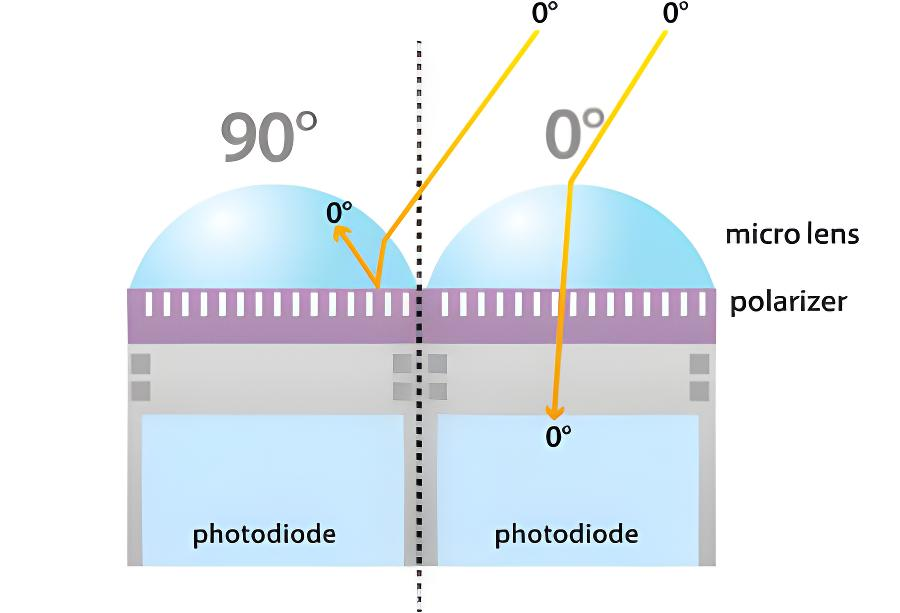
\includegraphics[width=0.48\textwidth]{figures/crosstalk_off_upscaled.jpg}
    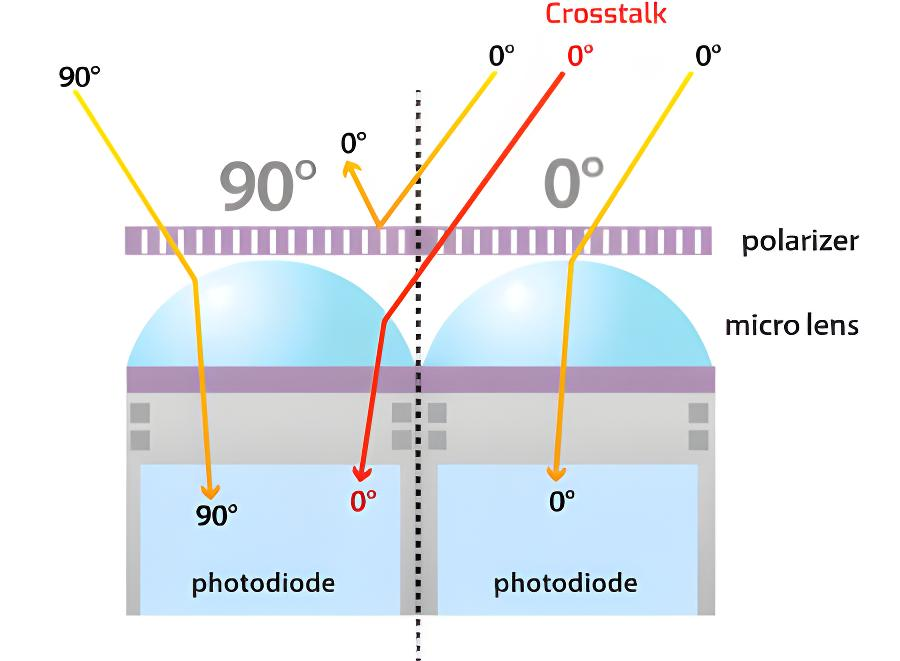
\includegraphics[width=0.48\textwidth]{figures/crosstalk_upscaled.jpg}
    \caption{Polarizer developed by Sony (left) to ensure low crosstalk between pixels \cite{lucidvisionlabsPolarizationExplainedSony2018}.}
    \label{fig:camera_crosstalk}
\end{figure}
\glspl{pg} can be formed from groups of four pixels with different filter angles, allowing the capture in practice to capture four pictures simultaneously with angles of polarization.
A Bayer Pattern can be added on top of this, resulting in groups of 16 pixels called \glspl{cpg}, enabling the capture of color information as well.
This configuration is referred to as a \gls{cpfa} and is illustrated in Figure \ref{fig:polarization_naming}.

\begin{figure}[H]
    \centering
    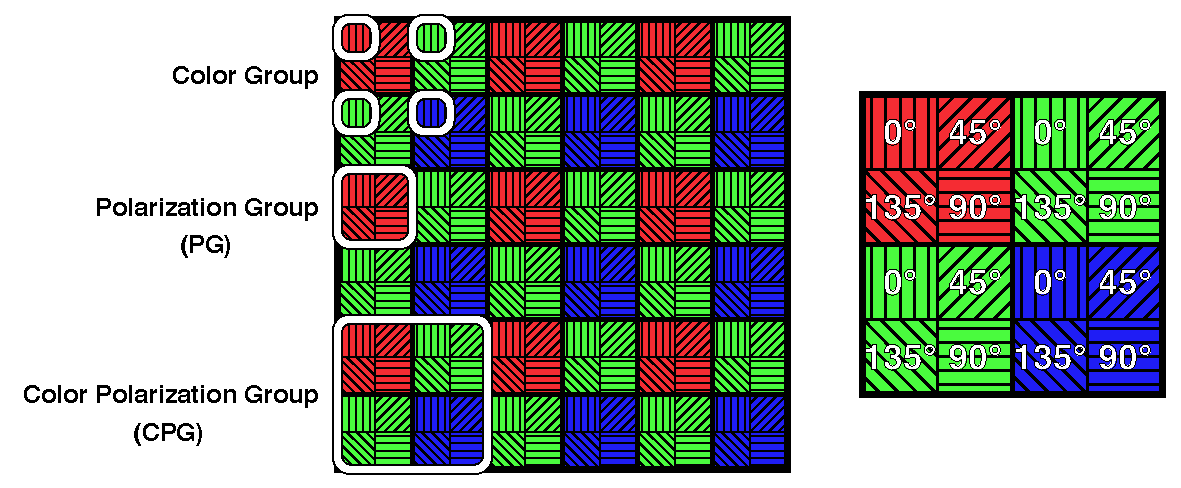
\includegraphics[width=\textwidth]{figures/polarized_image/naming.pdf}
    \caption{Naming convention for the different polarization angles.}
    \label{fig:polarization_naming}
\end{figure}

\subsection{Stokes Parameters}
Given the four polarisation angles, the Stokes parameters can be calculated \cite{piascoSurveyVisualBasedLocalization2018}.
With these parameters, the \gls{dolp} and \gls{aolp}, which is the angle of polarization relative to the camera, can be calculated as follows \cite{piascoSurveyVisualBasedLocalization2018}:
\begin{align}
    S_0 =  & I_0 + I_{90}                                                      \\
    S_1 =  & I_0 - I_{90}                                                      \\
    S_2 =  & I_{45} - I_{135}                                                  \\
    DoLP = & \frac{\sqrt{S_1^2 + S_2^2}}{S_0}  \label{eq:dolp}                 \\
    AoLP = & \frac{1}{2} \arctan{\left(\frac{S_2}{S_1}\right)} \label{eq:aolp}
\end{align}

A common way to visualize this is to encode the \gls{aolp} as hue and the \gls{dolp} as the value in the \gls{hsv} color space.
This can either be done for the three color channels separately or after calculating the grayscale value, which is illustrated in Figure \ref{fig:polarization_visualization}, which is captured by the \sr.
The benefits of polarization are evident in this image, as the water surface has a high \gls{dolp} and predictable \gls{aolp}.
The benefits and limitations of this polarization information are further discussed in Section \ref{sec:pol_benefits}.

\begin{figure}[H]
    \centering
    \subcaptionbox{The four polarization channels with $0^\circ$, $45^\circ$, $90^\circ$ and $135^\circ$ polarization angle respectively.}{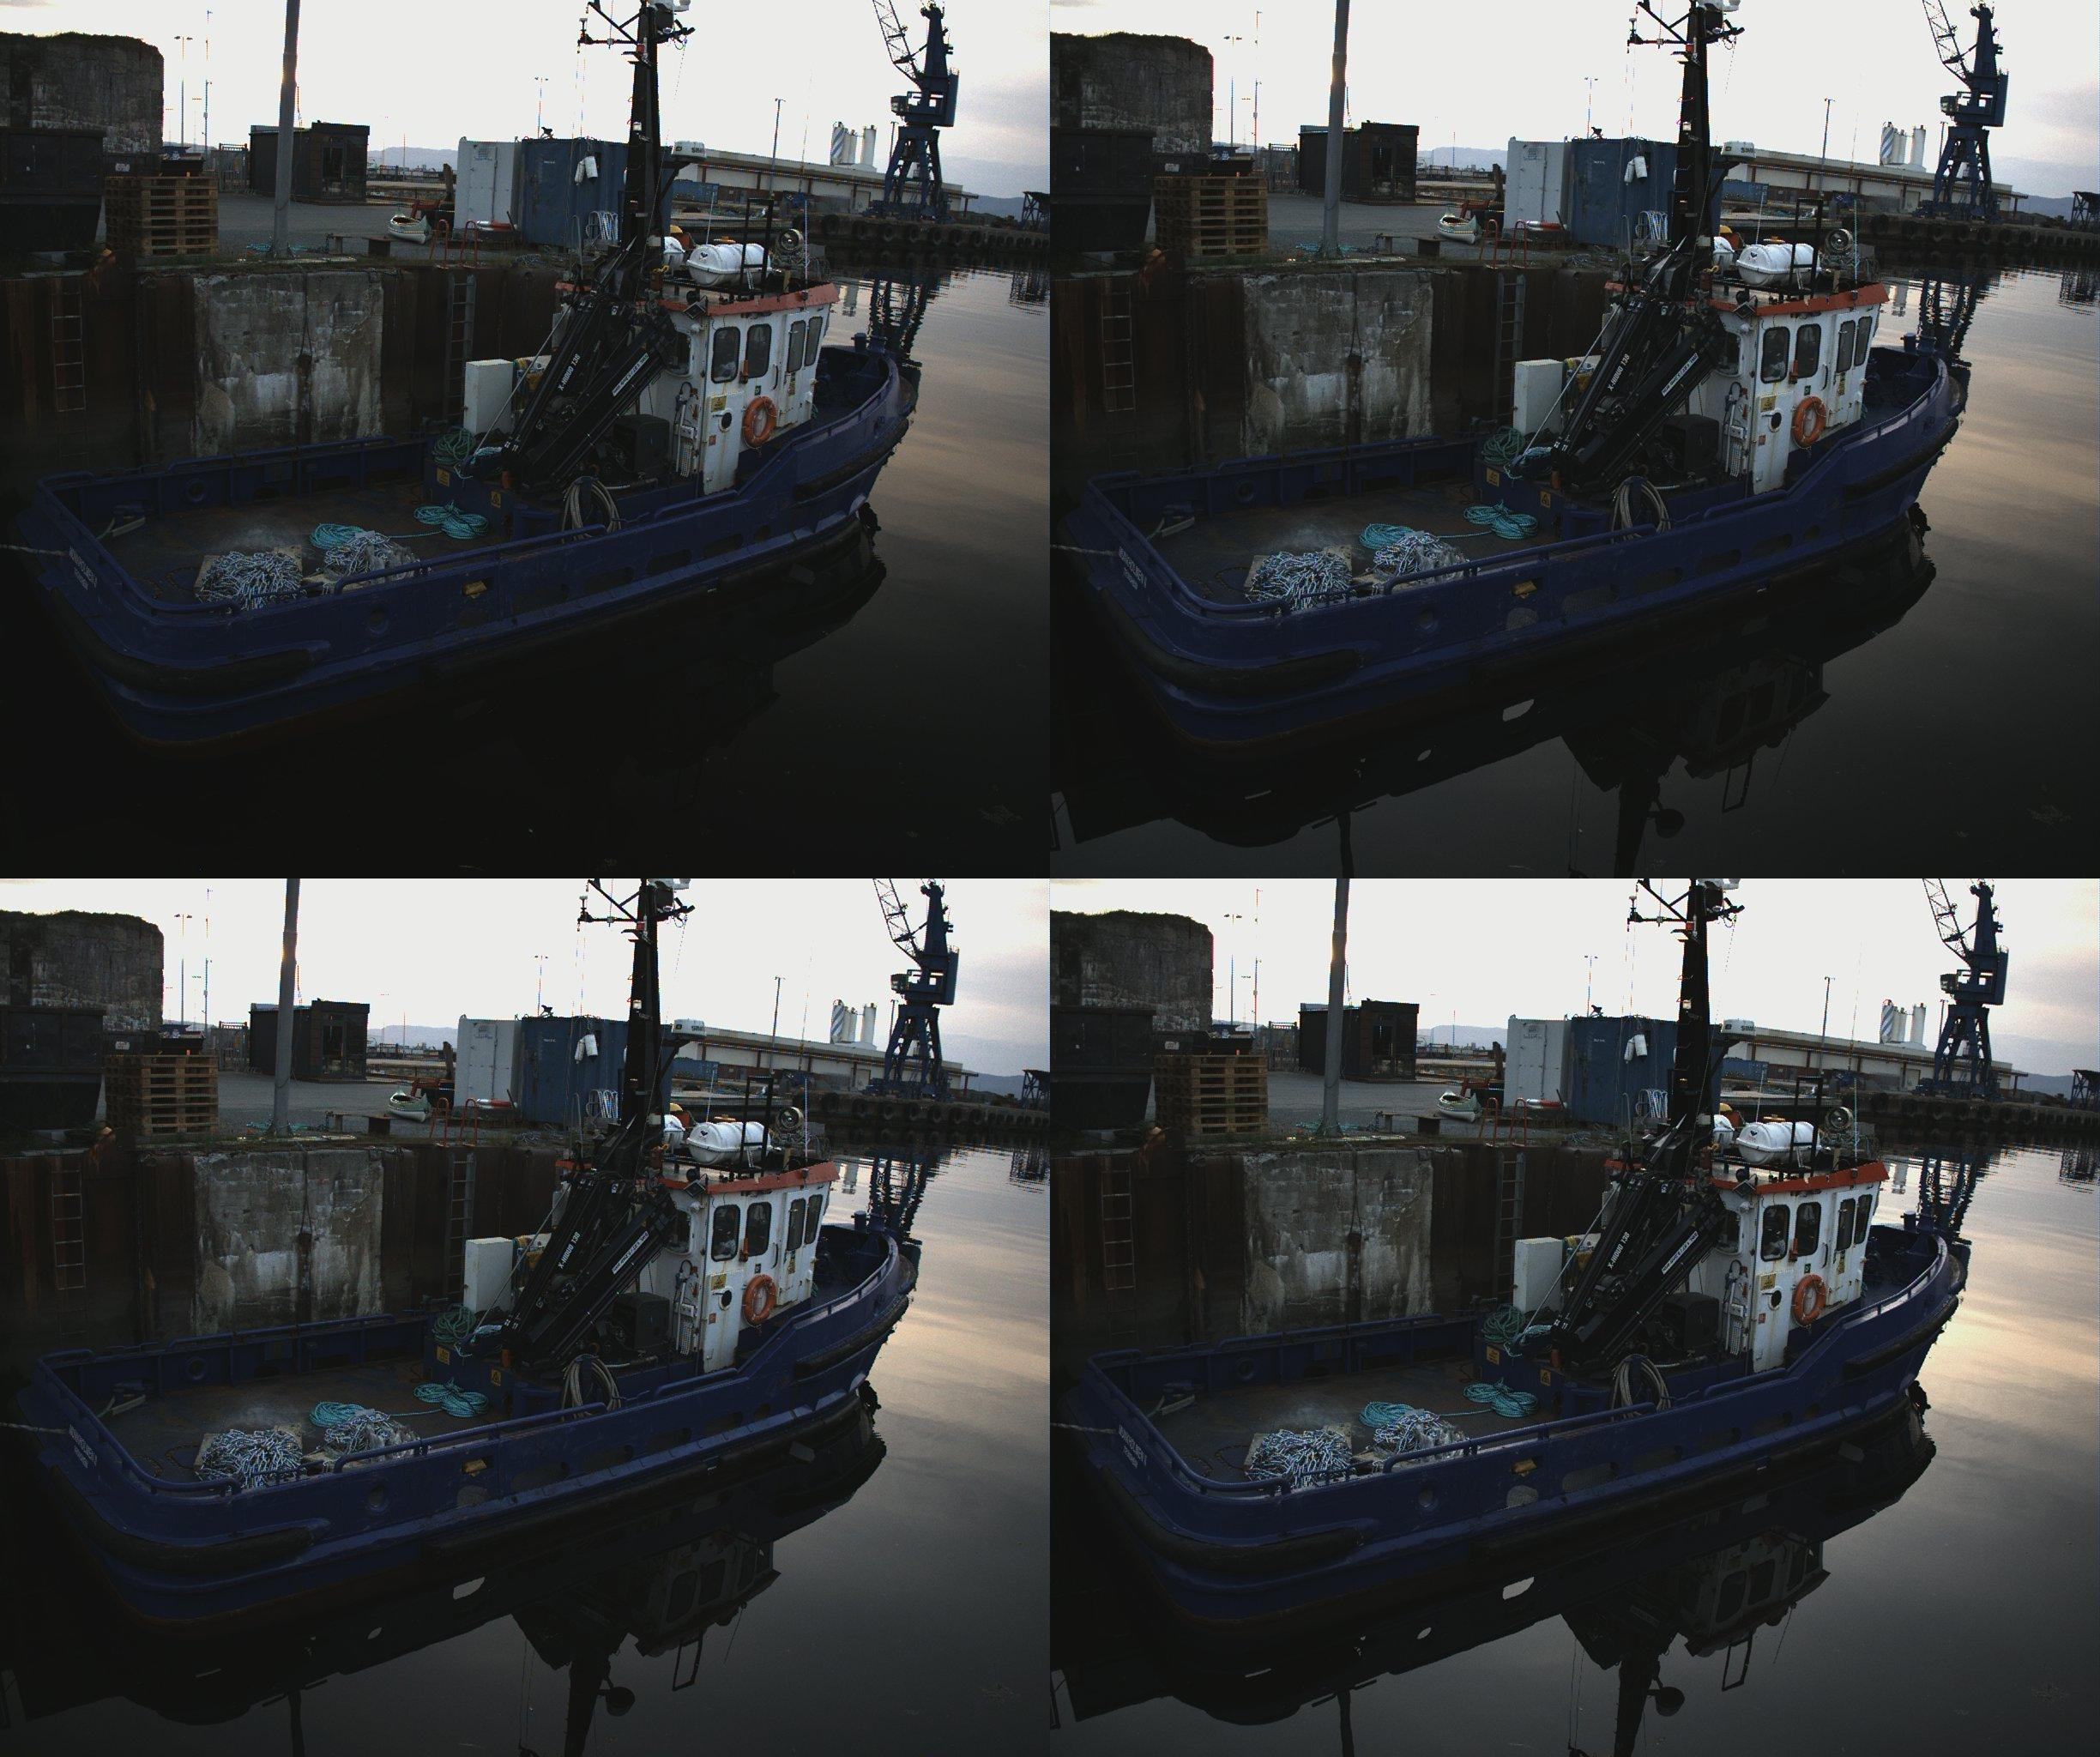
\includegraphics[width=.8\textwidth]{figures/pictures/img_00231_split.jpeg}}
    \subcaptionbox{\gls{aolp} and \gls{dolp} visualized as hue and value.}{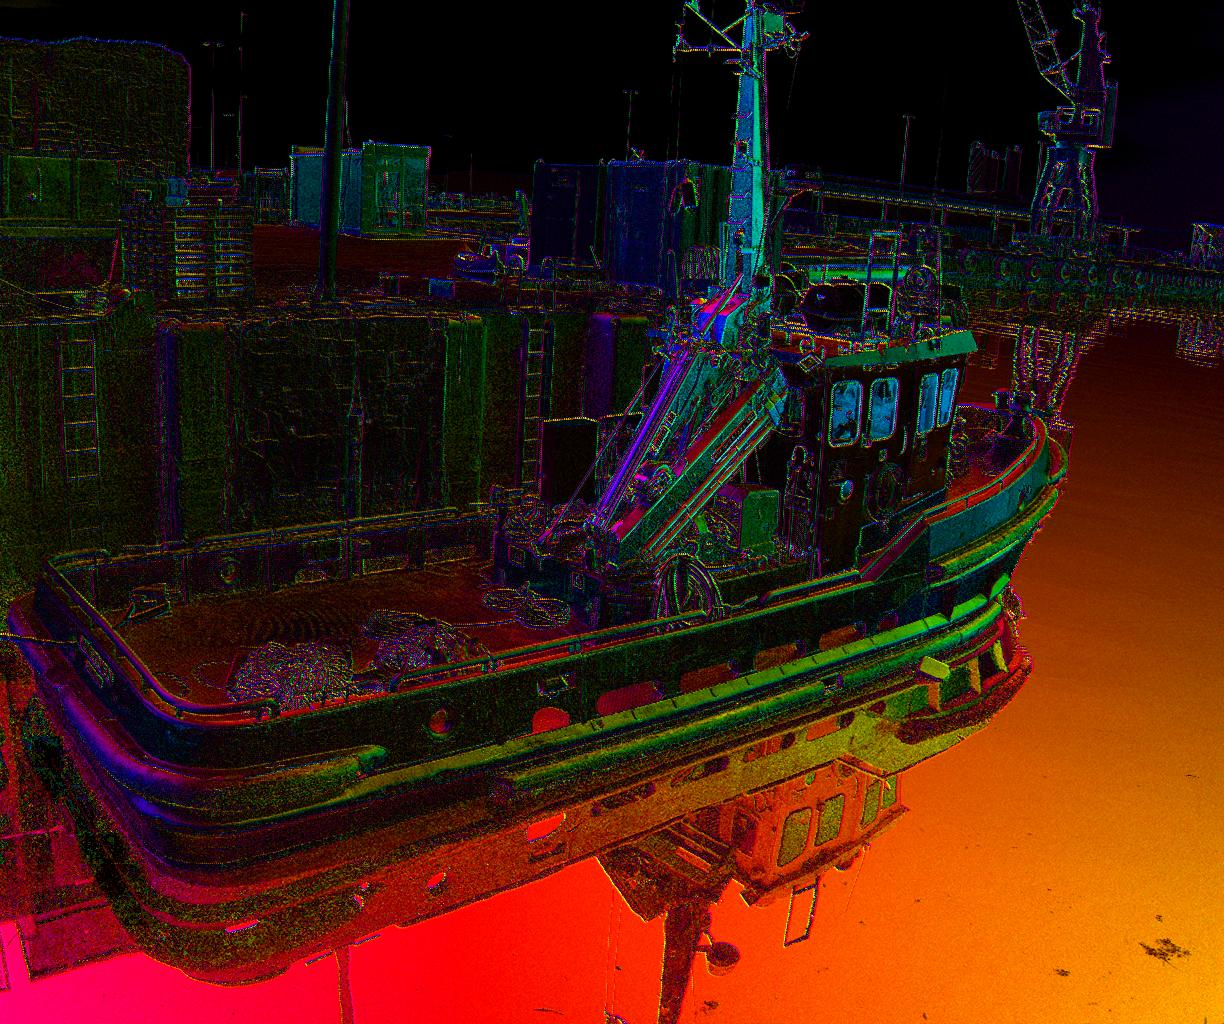
\includegraphics[width=.8\textwidth]{figures/pictures/aolp_left_231.jpeg}}
    \caption{Visualization of a \gls{cpfa} sensor.}
    \label{fig:polarization_visualization}
\end{figure}




\section{Triton Polarization Camera}
The \sr is equipped with two Triton 5.0 MP Polarization cameras that use the IMX264MYR \gls{cpfa} sensor from Sony.
The \cams are configured by setting the value of \code{nodes} in four different \code{nodemaps}, presented in Table \ref{tab:nodemaps} \cite{lucidvisionlabsTritonMPPolarized2020}.

A lot of time was spent trying out different parameters.
This was initially a tedious process as it had to be done using strings.
I extended the API by creating a wrapper around each \code{nodemap} to make this process faster.
The wrapper defines each node as a \py class, making it easy to set and read each node's values as all the possible values are defined in the class.
This was done by systematically querying the nodemaps for all their available nodes, parsing the descriptions values, and generating \py classes using \gls{jinja} templating.

\begin{minted}{python}
    nodemap["PixelFormat"] = "BayerRG10p" # Default
    wrapped_nodemap.PixelFormat.set_BayerRG10p() # Wrapper
\end{minted}
\begin{table}[H]
    \centering
    \small
    \begin{tabular}{|l|c|l|}
        \hline
        \textbf{Nodemap} & \textbf{\# of nodes} & \textbf{Description}                    \\
        \hline
        \code{device}    & 417                  & Camera parameters i.e. sutter speed.    \\
        \code{interface} & 22                   & Network parameters, i.e. network masks  \\
        \code{stream}    & 24                   & Stream params, i.e. resend policy       \\
        \code{system}    & 36                   & System parameters, i.e. thread priority \\
        \hline
    \end{tabular}
    \caption{Number of nodes in each nodemap.}
    \label{tab:nodemaps}
\end{table}



\subsection{Bugs in the firmware and documentation}
In certain instances, the \gls{api} would correctly throw errors if an incorrect value was set or if a value couldn't be temporarily written, such as attempting to set the gain while it was in automatic mode. However, there were cases where the \gls{api} didn't provide any warnings or errors, yet the value wasn't successfully set. This led to confusion, especially while configuring the trigger source, as it would be ignored if the \cam was already in trigger mode.

Additionally, there are certain mistakes in the documentation provided by Lucid. One such mistake is the claim that the cameras support the use of \gls{lut}. However, after conducting a thorough search and receiving confirmation via email, it was established that \gls{lut} is unfortunately not supported by the cameras \cite{fischerRe15406LUT2022} \cite{lucidvisionlabsTritonMPPolarized2020}.

\section{Synchronization (PPT+PPS)}
\gls{ptp} synchronization is utilized to synchronize the two cameras.
To verify the synchronization, the cameras were configured to pull the \textit{Line 2} \gls{gpio} pin high during the active exposure period, as indicated in Table \ref{tab:triton_pinout}.
This signal was then connected to an oscilloscope to measure the synchronization offset, which represents the time difference between the two cameras, as shown in Figure \ref{fig:sync_offset}.

In most cases, the synchronization offset varied between $\pm20\mu s$, but occasionally reached as high as $\pm50\mu s$.
Nevertheless, these values are within the acceptable range, as they are significantly lower than the exposure time, even when operating in daylight conditions.

The cameras also report their estimated \gls{ptp} offset, which partially aligned with the measured offset, but was not totally accurate.

\begin{table}
    \centering
    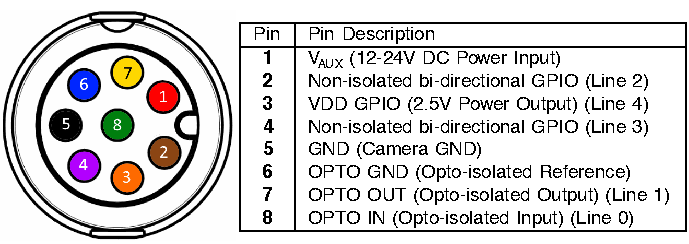
\includegraphics[width=\textwidth]{figures/triton_pinout.pdf}
    \caption{\cam \gls{gpio} connector \cite{lucidvisionlabsTritonMPPolarized2020}}
    \label{tab:triton_pinout}
\end{table}

\subsection{Reduce trigger latency}
It is possible to reduce the trigger latency of the cameras, which results in a lower synchronization offset.
This can be achieved by setting the \code{TriggerLatency} node to \code{OneLine}.
This reduces the average trigger offset down to $10\mu s$.
Unfortunately, this option becomes unavailable while the \code{TriggerOverlap} node is set to \code{set_PreviousFrame}, which is required to reach higher framerates.

\begin{figure}[H]
    \centering
    \subcaptionbox{Synchronization at $25ms$ resolution.
        \label{fig:sync_25us}}{
        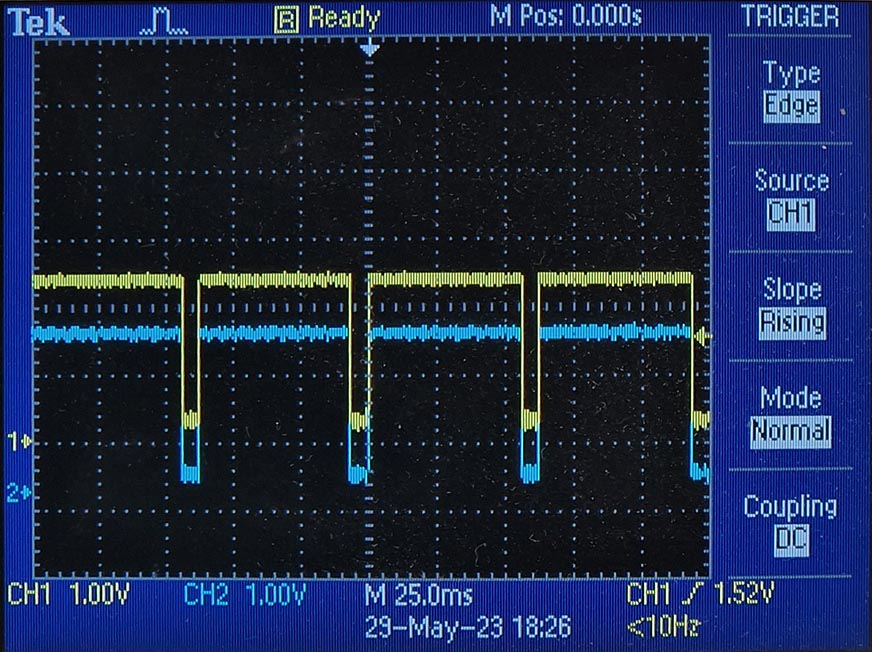
\includegraphics[width=0.8\textwidth]{figures/synchronization/ms.jpg}
    }
    \subcaptionbox{Synchronization at $10\mu s$ resolution.}{
        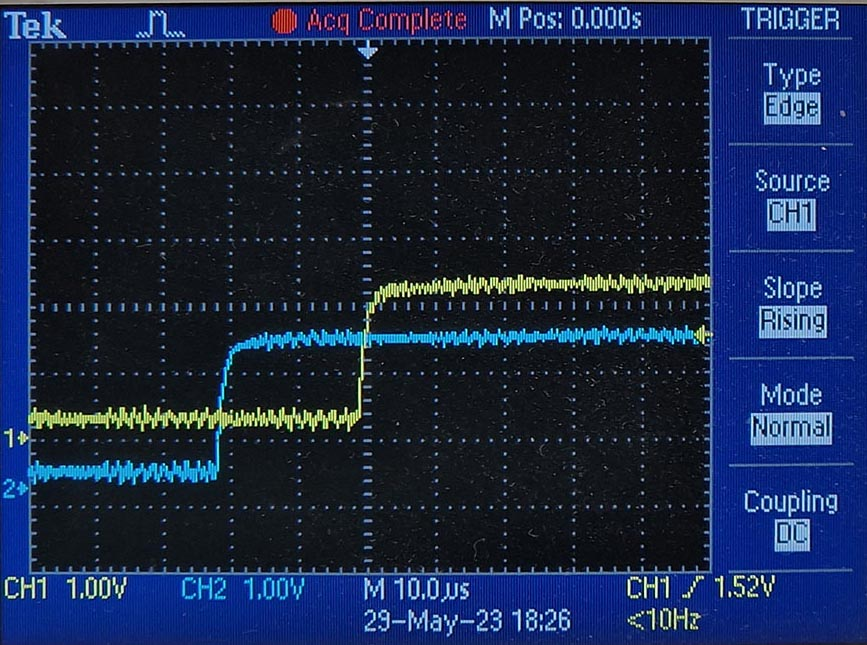
\includegraphics[width=0.8\textwidth]{figures/synchronization/us.jpg}
    }
    \caption{Measured synchronization offset of $22\mu s$ between the two cameras.}
    \label{fig:sync_offset}
\end{figure}


\section{Network configuration}
\label{sec:network_configuration}
The \jx has a built-in ethernet adapter and has been equipped with an extra WiFi adapter, as well as a network card consisting of four independent ethernet adapters \cite[Section 6.5]{martensPortableSensorRig2022}.
The following section presents relevant information about network configuration and outlines the steps to achieve a bandwidth of $1Gb/s$ on each of the four Ethernet adapters.

\paragraph{Link-Local Addresses (LLA)} are a commonly used in \gls{gigev} camera setups \cite{teledyneSettingIPAddress01} \cite{lucidvisionlabsArenaSoftwareDevelopment2020}.
It enables devices to automatically be assigned IP addresses without a specific subnet without relying on a \gls{dhcp} server or static IP \cite{annieahujaweb2020LinkLocalAddress2022}.
This directly connects a \gls{gigev} camera and an ethernet adapter without an intermediary router \cite{annieahujaweb2020LinkLocalAddress2022}.

As shown in Figure \ref{fig:lucid_ip_discovery}, the \cams are configured to use \gls{lla} if the use of Persistent IP and \gls{dhcp} fails \cite{lucidvisionlabsArenaSoftwareDevelopment2020}.
This is leveraged during the discovery process as discussed in Section \ref{sec:discovery}.

\paragraph{Static IP} is supported by the \cams, but I decided not to use this feature \cite{lucidvisionlabsArenaSoftwareDevelopment2020}.
The motivation to avoid this was to avoid the need to change the IP ranges of the network adapters and to keep the cameras in their factory default configuration, as this would make it easier to use them for other projects in the future.

\paragraph{Jumbo Frames} is a type of network frame that carries more payload than the standard \gls{mtu} size \cite{ieeeIEEEStandardsInterpretation2002} \cite{lucidvisionlabsJumboFramesLUCID2020}.
Increasing the maximal \gls{mtu} size typically leads to improved performance for high-bandwidth cameras.
It can also help reduce the CPU load on the host system, as there is less protocol overhead \cite{lucidvisionlabsJumboFramesLUCID2020} \cite{lukeThingsYouShould2018}.
Both the ethernet card used on the \jx as well as the \cams support Jumbo frames \cite{IntelI350am4Chip} \cite{lucidvisionlabsTritonMPPolarized2020}.
The \code{ifconfig <device> mtu 9000} command is used to enable jumbo frames on a device.

\begin{figure}[H]
    \centering
    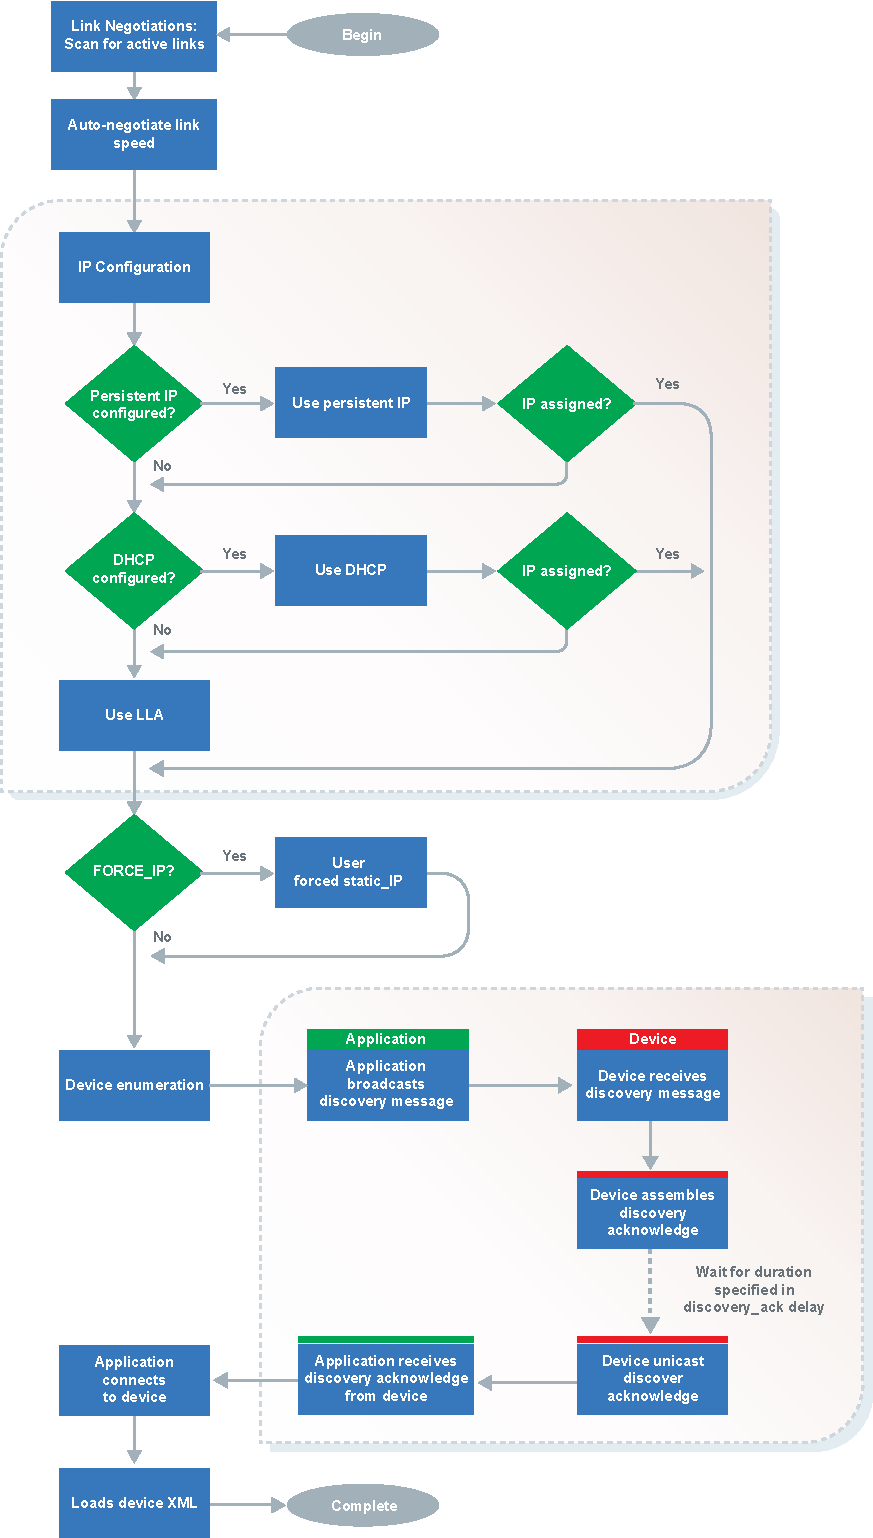
\includegraphics[height=\textheight]{figures/PDF/lucid_ip_discovery.pdf}
    \caption{Figure of the discovery and enumeration process of Lucid cameras \cite{lucidvisionlabsTritonMPPolarized2020}}
    \label{fig:lucid_ip_discovery}
\end{figure}


\paragraph{Receive Buffers} are storage areas where network packets are temporarily held before being processed by the \gls{cpu}, as depicted in Figure \ref{fig:linux_network} \cite{danQueueingLinuxNetwork2013}.
To enhance performance and prevent starvation, it is recommended to increase the default number of receive buffers, also known as \glspl{skb} \cite{lucidvisionlabsReceiveBuffers2020} \cite{danQueueingLinuxNetwork2013}.
On the \jx, the maximum number of receive buffers was raised from the default 256 to 4096 using the command \code{ethtool -G <device> rx 4096} \cite{danQueueingLinuxNetwork2013}.
Additionally, the maximum buffer size was permanently increased to $16MiB$ by adding the following lines to the \code{/etc/sysctl.conf} file \cite{redhat10ChangingNetwork}\cite{ibmIBMDocumentationTCPIP2021}:

\begin{minted}{bash}
net.core.rmem_default=16777216
net.core.rmem_max=16777216
\end{minted}

Expanding the number of buffers increases memory usage and may introduce additional latency as the queue grows longer, but in this case, it did not lead to any issues \cite{danQueueingLinuxNetwork2013}.

\begin{figure}[H]
    \centering
    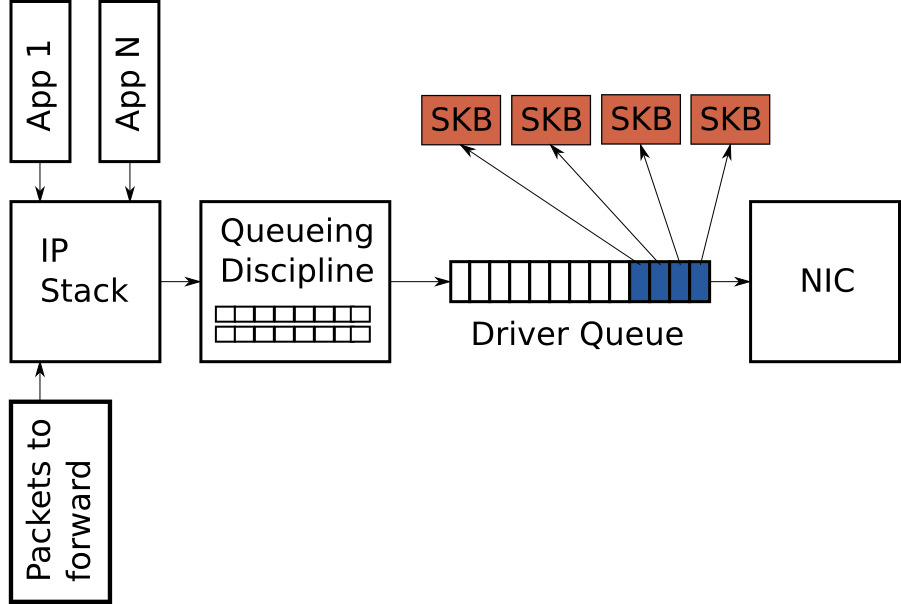
\includegraphics[width=0.8\textwidth]{figures/linux_networking.png}
    \caption{Simplified high-level overview of the queues on the transmit path of the Linux network stack \cite{danQueueingLinuxNetwork2013}}
    \label{fig:linux_network}
\end{figure}


\chapter{Conclusion}
In this \master I have successfully finished the development of a \sr capable of capturing synchronized stereo data from two polarization cameras.
Using \gls{cuda} and \gls{gstreamer} I have achieved on-the-fly hardware-accelerated video compression on the \jx, which enables the recording of longer data sets.
In addition to this, the \sr is now easy to use for anyone, thanks to the new web-based \gls{gui} and 3D printed ergonomic handles.

Completing the \sr has been a challenging but rewarding process where I have acquired many new skills.
Based on the experience I have gained, I can say that designing and building a \sr is a non-trivial and time-consuming task that should be avoided if existing datasets are sufficient for the task at hand.

The \sr provides a combination of sensor data that is believed to be unique and valuable for future research.
My supervisor, Annette Stahl, and I have started planning a scientific paper presenting this new type of data set and how stereo polarization cameras can be used to enhance situational awareness in the maritime domain.

The achievements of this \master are expected to be an excellent starting point for my future Ph.D. work and be used in several other projects at NTNU.




\newglossarystyle{mystyle}{\glossarystyle{long}\renewenvironment{theglossary}%
    {\footnotesize \begin{longtable}{p{3cm}p{\glsdescwidth}}}{\end{longtable}}%
}
\printglossary[style=mystyle,type=\acronymtype]
\printglossary[style=mystyle]
\AtNextBibliography{\footnotesize}
\printbibliography

\chapter{Additional resources}
\label{chap:additional_resources}
\section{Index Table used to Determine Memory Access Pattern}
The following table was used to determine the correct access pattern in Section \ref{sec:contuguous_access}.
\begin{table}[H]
    \small
    \begin{tabular}{r|rrrrr|rrrrr}
        T  & $c_T[0]$ & $c_T[1]$ & $c_T[2]$ & $c_T[3]$ & $c_T[4]$ & $a_T[0]$ & $a_T[1]$ & $a_T[2]$ & $a_T[3]$ & $a_T[4]$ \\
        \hline

        0  & $0$      & $32$     & $64$     & $96$     & $128$    & $0$      & $1$      & $2$      & $3$      & $4$      \\
        1  & $1$      & $33$     & $65$     & $97$     & $129$    & $5$      & $6$      & $7$      & $8$      & $9$      \\
        2  & $2$      & $34$     & $66$     & $98$     & $130$    & $10$     & $11$     & $12$     & $13$     & $14$     \\
        3  & $3$      & $35$     & $67$     & $99$     & $131$    & $15$     & $16$     & $17$     & $18$     & $19$     \\
        4  & $4$      & $36$     & $68$     & $100$    & $132$    & $20$     & $21$     & $22$     & $23$     & $24$     \\
        5  & $5$      & $37$     & $69$     & $101$    & $133$    & $25$     & $26$     & $27$     & $28$     & $29$     \\
        6  & $6$      & $38$     & $70$     & $102$    & $134$    & $30$     & $31$     & $32$     & $33$     & $34$     \\
        7  & $7$      & $39$     & $71$     & $103$    & $135$    & $35$     & $36$     & $37$     & $38$     & $39$     \\
        8  & $8$      & $40$     & $72$     & $104$    & $136$    & $40$     & $41$     & $42$     & $43$     & $44$     \\
        9  & $9$      & $41$     & $73$     & $105$    & $137$    & $45$     & $46$     & $47$     & $48$     & $49$     \\
        10 & $10$     & $42$     & $74$     & $106$    & $138$    & $50$     & $51$     & $52$     & $53$     & $54$     \\
        11 & $11$     & $43$     & $75$     & $107$    & $139$    & $55$     & $56$     & $57$     & $58$     & $59$     \\
        12 & $12$     & $44$     & $76$     & $108$    & $140$    & $60$     & $61$     & $62$     & $63$     & $64$     \\
        13 & $13$     & $45$     & $77$     & $109$    & $141$    & $65$     & $66$     & $67$     & $68$     & $69$     \\
        14 & $14$     & $46$     & $78$     & $110$    & $142$    & $70$     & $71$     & $72$     & $73$     & $74$     \\
        15 & $15$     & $47$     & $79$     & $111$    & $143$    & $75$     & $76$     & $77$     & $78$     & $79$     \\
        16 & $16$     & $48$     & $80$     & $112$    & $144$    & $80$     & $81$     & $82$     & $83$     & $84$     \\
        17 & $17$     & $49$     & $81$     & $113$    & $145$    & $85$     & $86$     & $87$     & $88$     & $89$     \\
        18 & $18$     & $50$     & $82$     & $114$    & $146$    & $90$     & $91$     & $92$     & $93$     & $94$     \\
        19 & $19$     & $51$     & $83$     & $115$    & $147$    & $95$     & $96$     & $97$     & $98$     & $99$     \\
        20 & $20$     & $52$     & $84$     & $116$    & $148$    & $100$    & $101$    & $102$    & $103$    & $104$    \\
        21 & $21$     & $53$     & $85$     & $117$    & $149$    & $105$    & $106$    & $107$    & $108$    & $109$    \\
        22 & $22$     & $54$     & $86$     & $118$    & $150$    & $110$    & $111$    & $112$    & $113$    & $114$    \\
        23 & $23$     & $55$     & $87$     & $119$    & $151$    & $115$    & $116$    & $117$    & $118$    & $119$    \\
        24 & $24$     & $56$     & $88$     & $120$    & $152$    & $120$    & $121$    & $122$    & $123$    & $124$    \\
        25 & $25$     & $57$     & $89$     & $121$    & $153$    & $125$    & $126$    & $127$    & $128$    & $129$    \\
        26 & $26$     & $58$     & $90$     & $122$    & $154$    & $130$    & $131$    & $132$    & $133$    & $134$    \\
        27 & $27$     & $59$     & $91$     & $123$    & $155$    & $135$    & $136$    & $137$    & $138$    & $139$    \\
        28 & $28$     & $60$     & $92$     & $124$    & $156$    & $140$    & $141$    & $142$    & $143$    & $144$    \\
        29 & $29$     & $61$     & $93$     & $125$    & $157$    & $145$    & $146$    & $147$    & $148$    & $149$    \\
        30 & $30$     & $62$     & $94$     & $126$    & $158$    & $150$    & $151$    & $152$    & $153$    & $154$    \\
        31 & $31$     & $63$     & $95$     & $127$    & $159$    & $155$    & $156$    & $157$    & $158$    & $159$
    \end{tabular}
    \caption{Relative location of image data stored in local memory. \newline e.g. \quad $a_1[1]=d[6+k]$ and  $c_1[1]=d[33+k]$.}
    \label{table:memory_index}
\end{table}
\section{Forum posts on PPS and compilation}\label{appendix:form_posts}

Following is a list of forum posts that were consulted during the compilation process.
The list is made by downloading and parsing the HTML from my activity log on the \gls{nforum} \cite{martensPostsRedEmil} and filtering out the relevant posts.
Out of the 544 posts visted, the 89 posts below matced one or more of the following regex search patterns:
\begin{itemize}
    \item \code{[^\w]pps}
    \item \code{boot}
    \item \code{flash}
    \item \code{kernel}
\end{itemize}
The total number of replies red is 1092.
Each post can be found by replacing the \code{<ID>} in the link below with the ID in the table.

\url{https://forums.developer.nvidia.com/t/<ID>}

\small
\begin{longtable}{p{.75\textwidth}rr}
    Title                                                                                               & Replies & ID     \\
    \hline                                                                                                                 \\
    AGX Xavier PPS fetch timeout R35.2.1(R32.7.1 works fine)                                            & 2       & 252374 \\
    About Flashing to a USB Drive                                                                       & 61      & 219316 \\
    Add PPS signal from gnss reciever to xavier nx                                                      & 11      & 155347 \\
    Add PPS signal to device tree in Nano                                                               & 5       & 169488 \\
    Boot Jetson AGX Xavier directly with configured SSD storage                                         & 11      & 219030 \\
    Boot from external drive                                                                            & 27      & 182883 \\
    Build the Real-Time Kernel                                                                          & 29      & 229571 \\
    CUDA 10.2 (cudart.so.10.2) missing (?) after FLASH install                                          & 9       & 186995 \\
    Can not flash Jetson xavier NX                                                                      & 6       & 183968 \\
    Can’t enable PPS in TX2 NX                                                                          & 8       & 196937 \\
    Can’t enable PPS on AGX Xavier                                                                      & 8       & 246834 \\
    Can’t enable PPS on Jetson AGX Xavier                                                               & 2       & 243842 \\
    Can’t find kernel\_src.tbz2                                                                         & 6       & 43288  \\
    Connecting GPS with PPS to Xavier                                                                   & 17      & 69356  \\
    Custom kernel build on Jetson AGX Xavier                                                            & 11      & 197023 \\
    Enable PPS on Jetson AGX Xavier                                                                     & 6       & 161342 \\
    Enable PPS on Jetson Linux 35.3.1 for Xavier AGX                                                    & 5       & 252416 \\
    Enabling PPS on Jetson Nano with Jetpack 4.3                                                        & 20      & 119418 \\
    Enabling PPS on Xavier AGX                                                                          & 31      & 147762 \\
    Error flashing SSD: /Linux\_for\_Tegra/bootloader/signed/flash.idx is not found                     & 3       & 240046 \\
    Error when flashing an NVMe ssd with initrd                                                         & 5       & 192031 \\
    Error: ECID read failed when using nvautoflash.sh                                                   & 3       & 212606 \\
    Facing problem while flashing the eMMC on the Jetson Nano production ready module (not the Dev Kit) & 28      & 80071  \\
    Failed to start Load Kernel Modules on Jetson Nano 4GB - L4T 32.7.2                                 & 8       & 223858 \\
    First Boot endlessly in “A start job is running for End-user configuration…”                        & 4       & 158015 \\
    Flash Issue - The target is in a bad state                                                          & 17      & 193746 \\
    Flash Jeston AGX Xavier with Command-Line Install with Docker on Windows 10 failed                  & 4       & 191870 \\
    Flash Jetpack 5.0.2 to SATA SSD                                                                     & 4       & 230802 \\
    Flash Jetson Agx Xavier Devkit to boot from SD Card                                                 & 9       & 196130 \\
    Flash jetpack 4.6 into sd card                                                                      & 4       & 194387 \\
    Flash kernel image on Nvidia TX2                                                                    & 7       & 60919  \\
    Flash of NVMe SSD                                                                                   & 7       & 189770 \\
    Flashing QSPI-NOR                                                                                   & 8       & 194180 \\
    Flashing Xavier with modified Device Tree                                                           & 11      & 80016  \\
    Flashing for booting from NVMe                                                                      & 7       & 210660 \\
    Flashing to NVMe SSD                                                                                & 9       & 210573 \\
    How to Boot from USB Drive?                                                                         & 50      & 172676 \\
    How to rebuild kernel for Jetson Linux 35.2.1                                                       & 5       & 243841 \\
    How to update cuda on TX2 without re-flashing TX2                                                   & 7       & 83298  \\
    How to use To use TEGRA\_AON\_GPIO in the kernel tegra x1??                                         & 5       & 68964  \\
    I try to flash nvme on my xavier nx, but failed and nothing on nvme                                 & 9       & 203664 \\
    Install kernel modules error"No rule to make target'modules\_install'. stop"                    & 6       & 214777 \\
    Is it possible to get a PPS output?                                                                 & 2       & 244787 \\
    JetPack 3.1 kernel source tag problem                                                               & 70      & 51929  \\
    JetPack 4.2 Flashing Issues and how to resolve                                                      & 67      & 73387  \\
    JetPack 5 and PPS on the Xavier NX                                                                  & 4       & 225824 \\
    JetPack 5.0.2,Orin AGX dev kit, /dev/pps1 not found                                                 & 11      & 230419 \\
    JetPack SDK in Docker for simple and clean flashing of a Jetson TX2                                 & 2       & 120526 \\
    Jetpack 4.2.1 fails to boot on Nano                                                                 & 9       & 78710  \\
    Jetpack 5.0.1 switch from Tegra 23x to 19x family SOC in kernel configuration                       & 2       & 219556 \\
    Jetpack 5.0.2 , boot from SATA SSD on Jetson Xavier NX. error: dev/sda1 not found                   & 27      & 238718 \\
    Jetpack-5.0.2 - Failed to flash NVMe with custom dtb and kernel’s Image                             & 8       & 238855 \\
    Jetpack5.0.2 kernel compile error                                                                   & 7       & 224160 \\
    Jetson Nano - Keeping time updated after reboot                                                     & 10      & 72380  \\
    Jetson TX2 failed to flash with unbuntu with SDK manager                                            & 3       & 185770 \\
    Jetson Xavier AGX 32GB flashing fails                                                               & 22      & 166931 \\
    Jetson Xavier AGX not booting after fstab modification                                              & 4       & 165516 \\
    Jetson Xavier Boot on SSD with Cboot                                                                & 20      & 73125  \\
    Jetson Xavier NX DEVKIT secureboot enabled                                                          & 21      & 158361 \\
    Jetson Xavier hardware pps\_out                                                                     & 18      & 124003 \\
    Jetson nano boot failed                                                                             & 7       & 73877  \\
    Jetson nano: PPS GPIO interrupt not getting registered                                              & 8       & 198085 \\
    Jetson tx2 cannot flash jetpack on wsl                                                              & 4       & 65739  \\
    Jetson xavier xn stuck in boot loop after trying to initrd flash to nvme SSD                        & 10      & 239392 \\
    Kernel build script nvbuild.sh with output dir option not working                                   & 3       & 173087 \\
    Move EMMC to NVMe boot: step 10 clarification                                                       & 5       & 188089 \\
    NTP with PPS Support on Xavier AGX                                                                  & 6       & 164887 \\
    New SDK Manager Flash Issue                                                                         & 6       & 81335  \\
    PPS kernel issue on Jetson Xavier AGX (L4T 34.1.1)                                                  & 5       & 224122 \\
    Please provide more detailed guidance to flash Jetson Nano with Windows 11 PC                       & 10      & 236808 \\
    Problem flashing AGX XAVIER                                                                         & 10      & 170912 \\
    R35.1 kernel + Tegra19x SOC family configuration compile errors                                     & 2       & 228026 \\
    Re-flash the device tree jetson agx xavier                                                          & 2       & 196565 \\
    Reboots while downloading the jetson-voice demo docker                                              & 5       & 125083 \\
    RuntimeError: CUDA error: no kernel image is available for execution on the device                  & 29      & 167708 \\
    SDK Manager flash to NVMe with flash checkpoint error                                               & 60      & 209375 \\
    Ssd boot on custom board with AGX SoM                                                               & 16      & 200732 \\
    System RAW image L4T 32.x.y l4t\_initrd\_flash.sh                                                   & 7       & 215356 \\
    TUTORIAL: Using sdkmanager for flashing on Windows via WSL2 + WSLg                                  & 2       & 225759 \\
    Unable to achieve PPS with Jetpack 5.0.2                                                            & 26      & 232101 \\
    Unable to flash Xavier AGX with SDK because of *** Reading ECID … *** Error: ECID read failed       & 2       & 189616 \\
    Unable to set breakpoints in kernels, debugging not working, VS2017 15.9.6                          & 5       & 70503  \\
    Using pps-gpio on Orin                                                                              & 3       & 225849 \\
    Xavier - Building the Kernel from Source                                                            & 2       & 77044  \\
    flash jetson tk1 using Windows                                                                      & 4       & 40331  \\
    how to setup NTPD with GPIO PPS                                                                     & 2       & 106942 \\
    keyword ‘return’ in cuda kernel what is its meaning?                                                & 5       & 19363  \\
    rootfsAB and test kernel/dtb                                                                        & 23      & 210108 \\
    “Cannot find matching device in recovery mode” error when flashing AGX Xavier                       & 21      & 219283
\end{longtable}



% \section{Compilation script}
\begin{minted}[fontsize=\tiny]{python}
    import subprocess
    from pathlib import Path
    import shutil
    import os
    from concurrent.futures import ThreadPoolExecutor, wait
    import requests
    
    password = input("Enter sudo password: ")
    
    
    def run(cmd: str, cwd=None):
        p = subprocess.run(cmd, cwd=cwd, env=env, shell=True, check=True)
        assert not p.returncode
    
    
    def run_sudo(cmd: str, cwd=None):
        p = subprocess.run(
            f"echo {password} | sudo -S {cmd}", cwd=cwd, env=env, shell=True, check=True
        )
        assert not p.returncode
        return p
    
    
    filedir = Path(__file__).parent
    dirs = [
        work_dir := filedir / "work",
        download_dir := filedir / "download",
        compiler_dir := work_dir / "l4t-gcc",
        l4t_dir := work_dir / "Linux_for_Tegra",
        public_dir := l4t_dir / "source/public",
        kernel_dir := l4t_dir / "source/public/kernel/kernel-5.10",
        rootfs_dir := l4t_dir / "rootfs",
        kernel_out := l4t_dir / "images",
        modules_out_dir := kernel_out / "modules",
        # sources_dir := l4t_dir / "sources",
    ]
    for d in dirs:
        d.mkdir(parents=True, exist_ok=True)
    
    
    cross_comp = compiler_dir / "bin/aarch64-buildroot-linux-gnu-"
    default_user_script = filedir / "l4t_create_default_user.sh"
    
    config = kernel_out / ".config"
    defconfig = kernel_dir / "arch/arm64/configs/defconfig"
    dtsi = (
        public_dir
        / "hardware/nvidia/soc/t19x/kernel-dts/tegra194-soc/tegra194-soc-base.dtsi"
    )
    pps_gpio_c = kernel_dir / "drivers/pps/clients/pps-gpio.c"
    
    env = os.environ.copy()
    env.update(
        {
            "CROSS_COMPILE": str(cross_comp),
            "LOCALVERSION": "-tegra",
            "TEGRA_KERNEL_OUT": str(kernel_out),
        }
    )
    
    
    def download(url: str, name: str):
        tmp_file = download_dir / f"tmp_{name}"
        if not (out_file := download_dir / name).exists():
            with requests.get(url, stream=True) as r, open(tmp_file, "wb") as f:
                shutil.copyfileobj(r.raw, f)
            shutil.move(tmp_file, out_file)
        return out_file
    
    
    common = "https://developer.nvidia.com/downloads/embedded/l4t/r35_release_v3.1"
    def get_bsp():
        url = f"{common}/release/jetson_linux_r35.3.1_aarch64.tbz2/"
        file = download(url, Path(url).name)
        run_sudo(f"tar -xjf {file} -C {work_dir}")
    
    def get_rootfs():
        url = f"{common}/release/tegra_linux_sample-root-filesystem_r35.3.1_aarch64.tbz2/"
        file = download(url, Path(url).name)
        run_sudo(f"tar -xjf {file} -C {rootfs_dir}")
    
    def get_bsp_sources():
        url = f"{common}/sources/public_sources.tbz2/"
        file = download(url, Path(url).name)
        run(f"tar -xjf {file}", work_dir)
        run("tar -xjf kernel_src.tbz2", l4t_dir / "source/public")
    
    def get_compiler():
        url = "https://developer.nvidia.com/embedded/jetson-linux/bootlin-toolchain-gcc-93"
        file = download(url, Path(url).name)
        run(f"tar -xf {file} -C {compiler_dir}")

    skipto = 0
    
    if skipto <= 0:
        futures = []
        with ThreadPoolExecutor() as executor:
            futures.append(executor.submit(get_bsp))
            futures.append(executor.submit(get_bsp_sources))
            futures.append(executor.submit(get_rootfs))
            futures.append(executor.submit(get_compiler))
            a, b = wait(futures)

    if skipto <= 1:
        for file in [pps_gpio_c, dtsi, defconfig]:
            shutil.copy(filedir / file.name, file)

    if skipto <=2:
        run("make mrproper", kernel_dir)
        kwargs = dict(
            ARCH="arm64",
            O=kernel_out,
            CROSS_COMPILE=cross_comp,
            KERNEL_OUT=kernel_out,
            LOCALVERSION="-tegra",
            INSTALL_MOD_PATH=str(kernel_out / "modules"),
        )
    
        common = f"make {' '.join(f'{k}={v}' for k, v in kwargs.items())} -j$(nproc)"
        run(f"{common} tegra_defconfig", kernel_dir)
        run(f"{common} Image", kernel_dir)
        run(f"{common} dtbs", kernel_dir)
        run(f"{common} modules", kernel_dir)
        run(f"{common} modules_install", kernel_dir)

    if skipto <=3:
        run_sudo(f"cp {kernel_out / 'arch/arm64/boot/Image'} {l4t_dir / 'kernel/'}")
        src = kernel_out / "arch/arm64/boot/dts/nvidia"
        dst = l4t_dir / "kernel/dtb"
        run_sudo(f"cp -a {src}/. {dst}")
    
    
    if skipto <=4:
        dst = l4t_dir / "kernel/kernel_supplements.tbz2"
        src = l4t_dir / "images/modules/lib/modules"
        dst.unlink(missing_ok=True)
        run_sudo(f"tar --owner root --group root -cjf {dst} {src}")
        run_sudo("/bin/bash apply_binaries.sh", l4t_dir)
        
    if skipto <=5:
        out = next((rootfs_dir).rglob("usr/lib/modules/*/kernel/drivers/gpu/nvgpu"))
        run_sudo(f"cp {kernel_out/'drivers/gpu/nvgpu/nvgpu.ko'} {out}")
        
        run_sudo(f"cp {default_user_script} {l4t_dir / default_user_script.name}")
        run_sudo(f"/bin/bash {l4t_dir / default_user_script.name} -p nvidia", l4t_dir)

    if skipto <=6:
        run_sudo("/bin/bash flash.sh jetson-agx-xavier-devkit mmcblk0p1", l4t_dir)

    if skipto <=7:
        file = l4t_dir / "tools/kernel_flash/l4t_initrd_flash.sh"
        layout = filedir / "flash_l4t_nvme.xml"
        size_gp = 520
        size_bytes = ((size_gp - 20) * 10**9 + 4096 - 1) // 4096 * 4096
        cmd = (
            f"/bin/bash {file} -c {layout}"
            " --external-device nvme0n1 --showlogs"
            " --no-flash"
            " --external-only"
            f" -S {size_bytes}"
            " jetson-agx-xavier-devkit nvme0n1p1"
        )
        run_sudo(cmd, l4t_dir)

    if skipto <=8:
        input("Put xavier into recovery mode and press enter")
        cmd = (
            f"/bin/bash {file} -c {layout}"
            " --external-device nvme0n1 --showlogs"
            " --flash-only"
            " --external-only"
            f" -S {size_bytes}"
            " jetson-agx-xavier-devkit nvme0n1p1"
        )
        run_sudo(cmd, l4t_dir)
\end{minted}
\section{Cura configurations}
\label{sec:cura_configurations}
Following is the complete set of parameters that were modified from their default values in Cura to achaive the desired print quality.
\begin{table}[H]
    \centering
    \scriptsize
    \begin{tabular}{ |l|r| }
        \hline
        \textbf{Parameter}               & \textbf{Value} \\
        \hline
        adhesion\_extruder\_nr           & 1              \\
        adhesion\_type                   & brim           \\
        bridge\_settings\_enabled        & False          \\
        jerk\_enabled                    & False          \\
        layer\_height                    & 0.16           \\
        layer\_height\_0                 & 0.3            \\
        material\_bed\_temperature       & 70             \\
        material\_shrinkage\_percentage  & 100            \\
        prime\_tower\_brim\_enable       & False          \\
        prime\_tower\_enable             & True           \\
        prime\_tower\_position\_x        & 220            \\
        prime\_tower\_size               & 20             \\
        support\_enable                  & True           \\
        support\_extruder\_nr            & 1              \\
        support\_interface\_extruder\_nr & 1              \\
        support\_type                    & buildplate     \\
        \hline
    \end{tabular}
    \caption{General configurations.}
\end{table}
\pagebreak
\begin{multicols}{2}
    \begin{table}[H]
        \scriptsize
        \begin{tabular}{ |l|r| }
            \hline
            \textbf{Parameter}                    & \textbf{Value} \\
            \hline
            acceleration\_print                   & 8000           \\
            acceleration\_roofing                 & 8000.0         \\
            acceleration\_topbottom               & 8000.0         \\
            acceleration\_travel                  & 8000.0         \\
            acceleration\_wall\_0                 & 8000.0         \\
            acceleration\_wall\_x                 & 8000.0         \\
            bottom\_layers                        & 5              \\
            bridge\_skin\_speed                   & 35.0           \\
            bridge\_wall\_speed                   & 35             \\
            brim\_gap                             & 0.4            \\
            brim\_line\_count                     & 10             \\
            cool\_fan\_speed                      & 60             \\
            cool\_min\_layer\_time                & 3              \\
            hole\_xy\_offset                      & 0.2            \\
            infill\_enable\_travel\_optimization  & True           \\
            infill\_pattern                       & trihex-        \\
                                                  & agon           \\
            infill\_sparse\_density               & 20             \\
            initial\_layer\_line\_width\_factor   & 120            \\
            jerk\_print                           & 30.0           \\
            material\_final\_print\_temperature   & 240.0          \\
            material\_flow\_layer\_0              & 75             \\
            material\_initial\_print\_temperature & 240.0          \\
            material\_standby\_temperature        & 240.0          \\
            prime\_tower\_min\_volume             & 5              \\
            retraction\_hop                       & 1.5            \\
            roofing\_layer\_count                 & 1              \\
            roofing\_monotonic                    & False          \\
            roofing\_pattern                      & lines          \\
            skin\_overlap                         & 10             \\
            speed\_infill                         & 70             \\
            speed\_layer\_0                       & 20             \\
            speed\_prime\_tower                   & 70.0           \\
            speed\_roofing                        & 70.0           \\
            speed\_topbottom                      & 70.0           \\
            speed\_wall\_0                        & 70.0           \\
            speed\_wall\_x                        & 70.0           \\
            support\_fan\_enable                  & False          \\
            support\_supported\_skin\_fan\_speed  & 60             \\
            support\_tree\_limit\_branch\_reach   & False          \\
            support\_xy\_distance\_overhang       & 0.4            \\
            switch\_extruder\_retraction\_amount  & 3              \\
            switch\_extruder\_retraction\_speed   & 40.0           \\
            switch\_extruder\_retraction\_speeds  & 40             \\
            top\_bottom\_pattern                  & lines          \\
            top\_bottom\_pattern\_0               & lines          \\
            top\_layers                           & 5              \\
            wall\_line\_count                     & 4              \\
            wall\_line\_width\_0                  & 0.42           \\
            xy\_offset                            & -0.05          \\
            xy\_offset\_layer\_0                  & -0.05          \\
            z\_seam\_x                            & 0              \\
            z\_seam\_y                            & 0              \\
            zig\_zaggify\_infill                  & True           \\
            \hline
        \end{tabular}
        \caption{Configurations of left extruder.}
    \end{table}
    \columnbreak
    \begin{table}[H]
        \scriptsize
        \centering
        \begin{tabular}{|l|r|}
            \hline
            \textbf{Parameter}                    & \textbf{Value} \\
            \hline
            acceleration\_topbottom               & 6000.0         \\
            acceleration\_wall\_0                 & 6000.0         \\
            acceleration\_wall\_x                 & 6000.0         \\
            brim\_line\_count                     & 8              \\
            initial\_layer\_line\_width\_factor   & 120            \\
            jerk\_print                           & 30.0           \\
            material\_final\_print\_temperature   & 215.0          \\
            material\_flow\_layer\_0              & 70             \\
            material\_initial\_print\_temperature & 215.0          \\
            material\_print\_temperature          & 215            \\
            material\_standby\_temperature        & 215.0          \\
            minimum\_bottom\_area                 & 1              \\
            minimum\_roof\_area                   & 0              \\
            minimum\_support\_area                & 10             \\
            prime\_tower\_min\_volume             & 6              \\
            skin\_monotonic                       & True           \\
            skirt\_brim\_speed                    & 20.0           \\
            speed\_infill                         & 70             \\
            speed\_layer\_0                       & 20.0           \\
            speed\_prime\_tower                   & 70.0           \\
            speed\_support                        & 70.0           \\
            speed\_topbottom                      & 70.0           \\
            speed\_wall\_0                        & 70.0           \\
            speed\_wall\_x                        & 70.0           \\
            support\_angle                        & 45             \\
            support\_bottom\_enable               & False          \\
            support\_interface\_density           & 100            \\
            support\_interface\_enable            & False          \\
            support\_interface\_offset            & 0              \\
            support\_offset                       & 1              \\
            support\_roof\_height                 & 0.5            \\
            support\_top\_distance                & 0              \\
            support\_tree\_angle\_slow            & 20             \\
            support\_tree\_top\_rate              & 35             \\
            support\_wall\_count                  & 2              \\
            support\_xy\_distance                 & 0.2            \\
            support\_xy\_distance\_overhang       & 0.1            \\
            support\_z\_distance                  & 0.1            \\
            switch\_extruder\_retraction\_amount  & 3              \\
            switch\_extruder\_retraction\_speed   & 40.0           \\
            switch\_extruder\_retraction\_speeds  & 40             \\
            top\_bottom\_pattern\_0               & con-           \\
                                                  & centric        \\
            xy\_offset\_layer\_0                  & -0.1           \\
            zig\_zaggify\_infill                  & True           \\
            \hline
        \end{tabular}
        \caption{Configurations of right extruder.}
    \end{table}
\end{multicols}


\end{document}
